\chapter{Workshop 6: How do we know it works?}\label{workshop-06}

\section{Match each claim to an observation}

Run \texttt{npm run verify}. The pinned companion edition typechecks and passes fifteen tests across its model/effect and presentation/application suites. The table below names the purpose of the evidence. The pseudo-terminal checks are retained separately because they exercise a real process and terminal device rather than the deterministic model.

\begin{center}
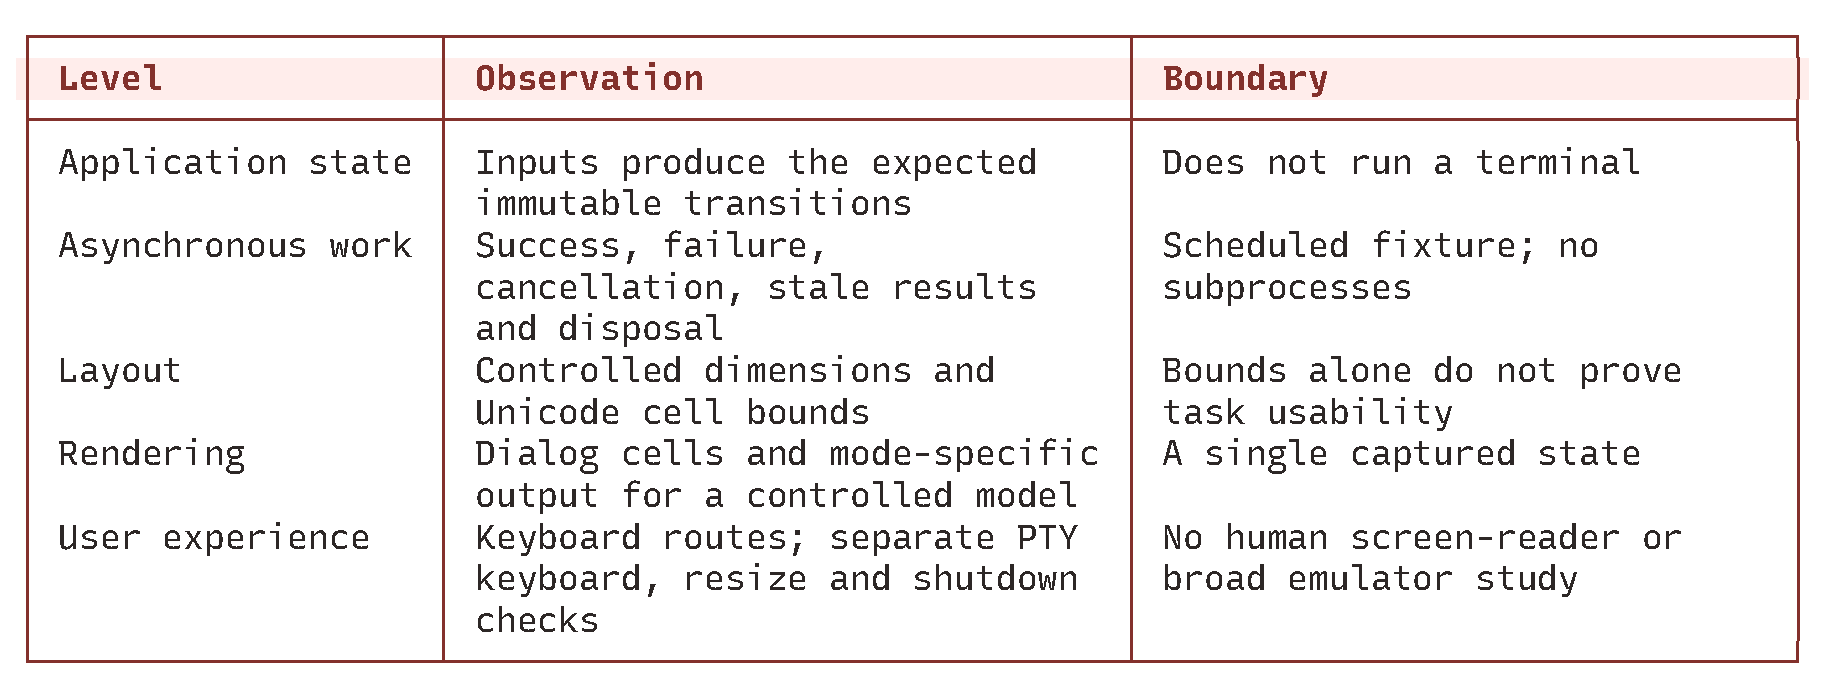
\includegraphics[width=\linewidth]{figures/tables/workshop-evidence-g1-1.pdf}
\par\smallskip{\scriptsize\color{BookMuted}Rows 1–5. Actual Bijou table component.}
\end{center}


\subsection{State and effects}

A state test starts a job, applies progress and checks the result. It also sends a late completion after cancellation and restart. This proves that the transition rejects the old run under those inputs. The scheduler test advances known delays, observes success and failure, cancels work and disposes the driver. It establishes which messages are emitted, including the absence of later messages after disposal.

Those tests do not establish the behavior of an operating-system process runner. The example has none. Replacing the scheduled fixture with subprocesses introduces buffering, exit codes, signal delivery and process-tree ownership that require their own adapter checks.

\subsection{Geometry and cells}

The layout test checks controlled widths and heights, including wide characters, combining text and an emoji sequence. The routing test supplies actual Bijou framework messages to the App and inspects the Surface produced for cancellation. These checks connect input, state and rendering. They still cannot tell whether a human notices the prompt, understands a failure message or can navigate effectively with a particular assistive tool.

\section{Read failure as information}

\subsection{Make the broken state reproducible}

The four exercise fixtures fail intentionally: modal input leaks, a stale result replaces current detail, a colored mark loses meaning, and work emits after closure. Each has a small command, a fixed starting state and an observable success criterion. The repaired path uses the production implementation. Default CI runs the ordinary suite and the repaired exercises; it does not mistake an intentionally broken teaching fixture for a regression in the final application.

\subsection{Avoid convenient evidence substitutions}

A typecheck does not establish a temporal property. A screenshot does not establish input ownership. A cell-bound test does not establish that every control remains reachable. A keyboard-routing test does not establish how a screen reader announces the application. Keep the attractive artifact and the behavioral evidence together while naming what each establishes.

\section{Read the decisions and their costs}

\subsection{Semantic styling}

The problem is a useful state disappearing when color disappears. A tempting shortcut is to make red mean failure by itself. The chosen starting point is textual state with optional visual reinforcement. This spends columns and can feel less compact. It preserves a fact that every mode can carry. Semantic tokens become useful when styling is added: the role remains ``error'' while a theme chooses its appearance.

\subsection{Explicit ownership}

The problem is an action reaching a page behind its dialog or a result reaching a screen that no longer owns it. Global shortcuts and unqualified callbacks look simple until those owners diverge. The chosen model makes input boundaries, run identities and view epochs explicit. The cost is more state and more transitions to test. The benefit is an ownership claim that can be examined before a convincing frame hides the defect.

\subsection{Meaning separate from presentation}

The problem is a consumer needing facts that were stored only as a rendered string. Keeping an immutable model and several formatters adds code paths and compatibility obligations. It also lets the same failed job appear in a table, a CI snapshot, TSV and explicit accessible prose without reconstructing its identity from decoration. Every added presentation must preserve the task's agreed facts; sharing a model does not make a formatter correct automatically.
